\chapter{Implementation}\label{ch:implementation}

This chapter focuses on the implementation of the offloading frameworks designed in \cref{ch:methodology}. In \cref{sec:offloading_framework}, it describes the implementation of the offloading framework in \gls{ros}. In \cref{sec:state_monitors}, it describes how the system states are measured for the robot and edge. 

% ------------------------------------------------------------
\section{Offloading Framework}\label{sec:offloading_framework}
% ------------------------------------------------------------

The offloading framework is implemented with \gls{ros}2 \cite{Macenski2022}. As mentioned in \cref{sec:frameworks_and_tools}, a \gls{ros} node is a process with a single purpose that communicates with other nodes through \gls{ros} communication patterns, such as topics and services. Therefore, different modules are implemented as \gls{ros} nodes and the communication between the nodes uses \gls{ros} topics exclusively, as illustrated in \cref{fig:ros_implementation}. The RGB images from the simulation are received by the offloading node via \gls{ros} topic. Thereon, the offloading node decides whether to offload to the edge or to compute it locally by publishing it to the corresponding \gls{ros} topics. The perception nodes receive the image from the \gls{ros} topics and publish the processed results to a dedicated \gls{ros} topic which is subscribed by a \gls{ros} bag recorder and will be eventually used for evaluation. Moreover, the network delays and the inference times are measured by the offloading node and the perception nodes by critical time points during the offloading and the inference. 

% figure for ROS implementation
\begin{figure}
    \centering
    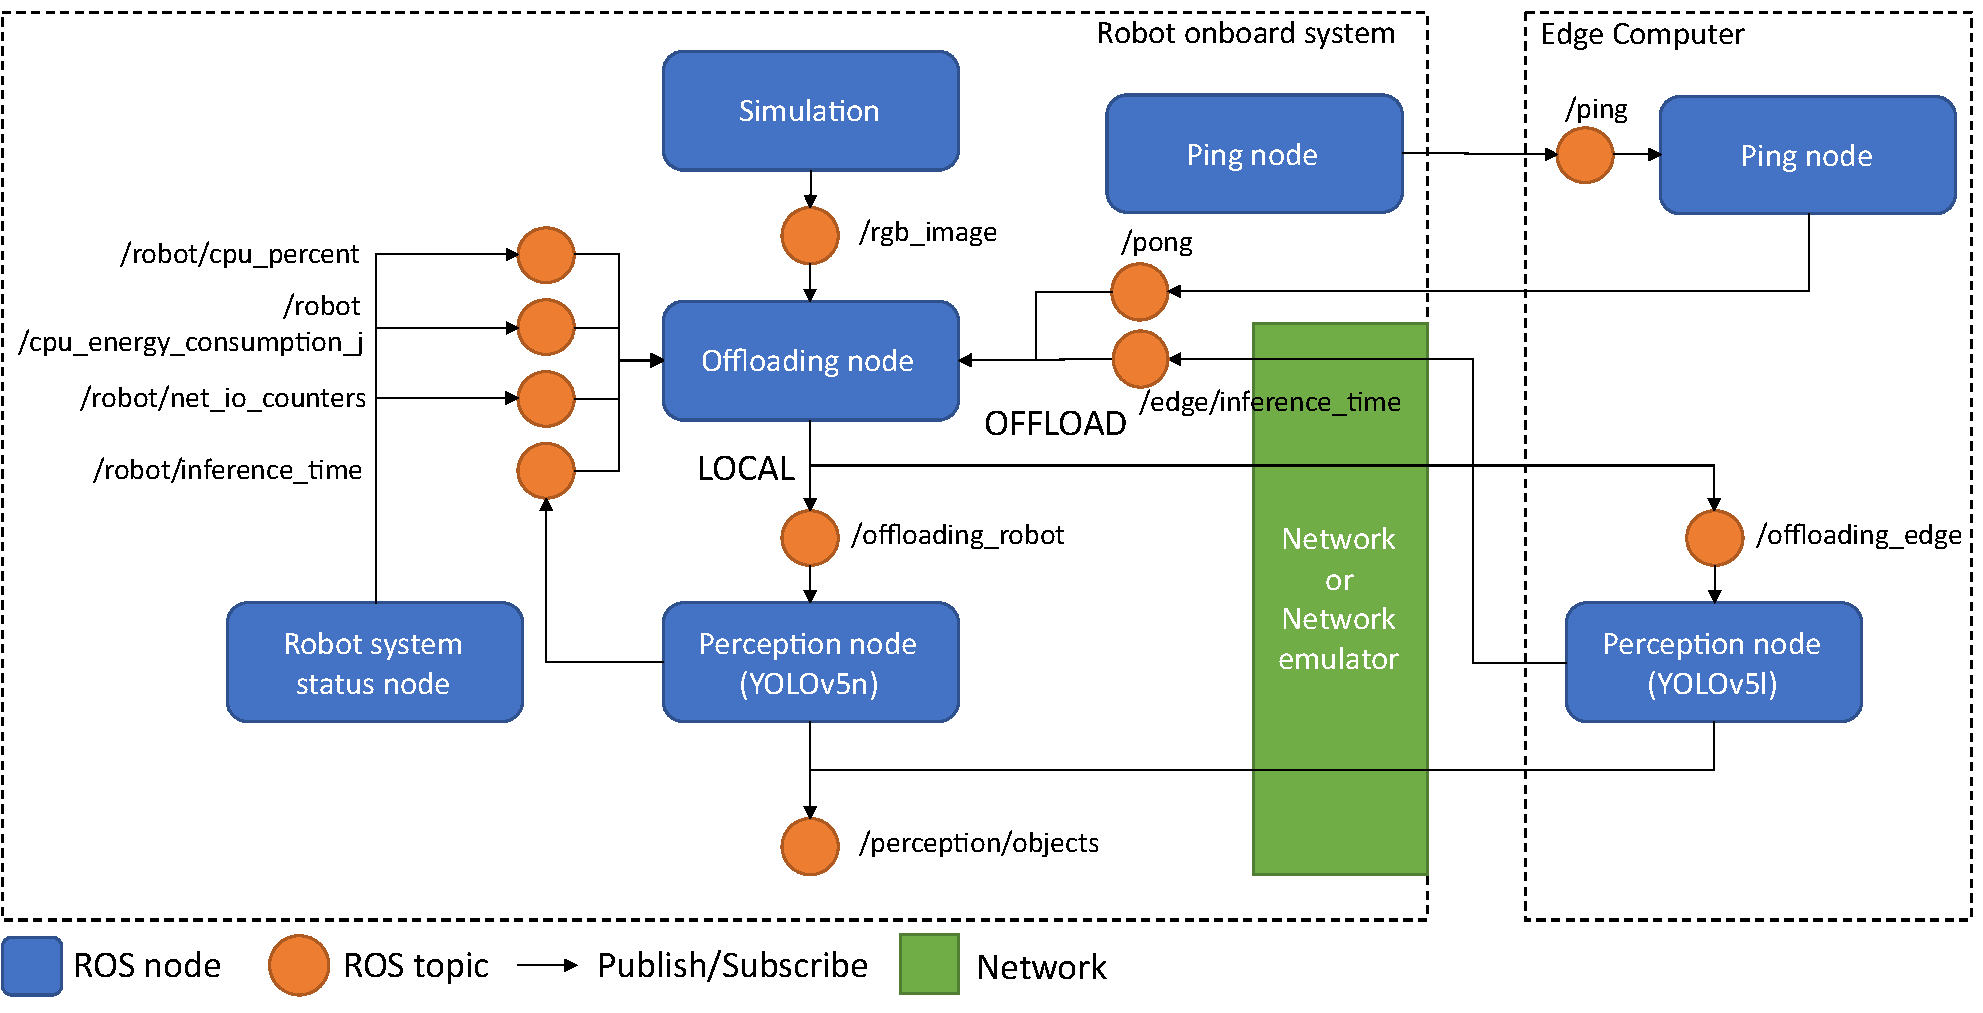
\includegraphics[width=\linewidth]{figures/setup/ros_implementation.pdf}
    \caption[Offloading framework implementation with \acrshort{ros}]{This figure shows the offloading framework implementation with \gls{ros}. Each blue block represents a \gls{ros} node. The orange circles represent \gls{ros} topics. The arrows show the direction of messages. The robot onboard system and the edge computer are separated by dotted rectangles. They can either be an actual physical system or a system virtualization such as a \gls{docker} container. The two systems can be connected by an actual network or a virtual network interface with \gls{netem} to emulate real network conditions.}
    \label{fig:ros_implementation}
\end{figure}

\subsection{Offloading Module}

% Add how is offloading module is implemented in ROS

The offloading node is the center of the offloading frameworks because it is responsible for making offloading decisions and carrying out the perception offloading. In order to keep track of the system states monitored by different nodes, the offloading node subscribes to different system state topics and stores the current states. To prevent the fluctuation in the systems states from affecting the offloading decision, the offloading node applies a \gls{sma} algorithm to smooth the data. The stored system states are passed to the offloading strategy during run time by the offloading node. In order to evaluate different offloading strategies, the offloading node uses a plugin mechanism to load the offloading strategy and hyper-parameters when the system first starts. 

\subsection{Perception Module}

% discuss the choice of synchronous inference and asynchronous inference. Also defend not retraining the model.

In general, an offloading task can be any computationally intensive algorithms an \gls{amr} is required to run, such as perception, navigation, \gls{slam}, path planning, etc. An object detection task based on RGB images is chosen as an example because it can have a significant performance difference between the robot's onboard system and the edge computer, which corresponds to the use cases of edge offloading. The robot is usually equipped with a simple onboard system with only access to \gls{cpu}, while edge computers are usually resource-abundant computers and data centers on-premise with access to \gls{gpu}, as described in \cref{sec:edge_computing}. As mentioned in \cref{sec:object_detection}, the robots use \glspl{dnn} to detect objects primarily. With frameworks like \gls{pytorch} and \gls{openvino} that can make use of \glspl{gpu}, the performance difference between \gls{amr}'s onboard system and the edge computer is immense. Therefore, object detection is chosen as an example for offloading tasks. 

% Table for inference time on different machines
\begin{table}[htb]%
    \centering%
    \begin{tabular}{lccccc}
        \toprule
        Model &                     YOLOv5n &   YOLOv5s &   YOLOv5m &   YOLOv5l &   YOLOv5x \\
        \midrule
        Robot inference time &      50.88 ms &  115.75 ms & 240.06 ms & 464.22 ms & 821.93 ms  \\
        Edge inference time &       8.87 ms &   11.51 ms &  20.35 ms &  31.18 ms &  52.55 ms  \\
        Model size \cite{Jocher2022} &                4 MB &      14 MB &     41 MB &     89 MB &     166 MB    \\
        \acrshort{map} \cite{Jocher2022} &                 45.7\% &    56.8\% &    64.1\% &    67.3\% &    68.9\%  \\
        \bottomrule
    \end{tabular}
    \caption{Inference times of different YOLOv5 models on \acrshort{amr}'s onboard system and edge computer}
    \label{tab:inference_time}%
\end{table}

In order to adapt to the performance difference between the \gls{amr}'s onboard system and the edge computer, the perception module should have two models available for object detection: a lightweight model that runs on the onboard system and a more complex model that runs on the edge computer. \gls{yolo}v5 provides a series of models with different complexities. To find appropriate models for the onboard system and the edge computer, the inference times of different models on different machines are investigated, which can be taken from \cref{tab:inference_time}. To simulate the discrepancy of the computation capabilities between the two systems, this experiment uses a \gls{nuc} equipped only with an Intel(R) Core(TM) i3-8109U \gls{cpu}. On the other hand, the edge computer is equipped with an Intel(R) Core(TM) i9-7900X \gls{cpu} and an Nvidia GeForce GTX 1060 6GB \gls{gpu}. The models are deployed with \gls{pytorch} and output an array of bounding box detection. The inference time is measured between the time when the \gls{yolo}v5 models receive the image and the time when the perception nodes output an array of bounding box detection. This includes the time for image pre-processing and the time of results post-processing. Furthermore, the image input for the offloading module has a frame rate of around 25 frames per second. The model sizes and the \gls{map} data are taken from the documentation from \citeauthor*{Jocher2022} \cite{Jocher2022}. The \gls{map} data are evaluated on \gls{coco} val2017 \cite{Lin2014}. As a compromise between the inference time and the performance, the \gls{yolo}v5n is chosen to be deployed on the \gls{amr}'s onboard system and \gls{yolo}v5l on the edge computer. 

The \gls{yolo}v5 models are deployed within the \gls{ros} nodes. Object detection is carried out in the perception nodes synchronously. This means the perception nodes are blocked during the execution of the inference. If the perception nodes cannot process the inference fast enough, the image messages will start to queue and the network delay will increase. The synchronous inference can achieve low inference time and reduce the \gls{cpu} usage of the perception nodes, since the \gls{ros} nodes do not have to spin continuously to check for processed results on another thread. The models are used in evaluation mode in \gls{pytorch} to reduce the overhead of the computation tasks used for training the models. The confidence threshold is set to 0.25 and the \gls{nms} threshold is set to 0.45 as the default settings of \gls{yolo}v5. Furthermore, the inference size is 640 by 640 pixels and the maximum number of detection per image is set to 1000. The inference is calculated in full precision, i.e., FP32. The detection classes are taken from the \gls{coco} data sets, provided by \gls{yolo}v5. 

% Move this part to limitation in conclusion chapter
% To delimit, the object detection models in use are pre-trained and not re-trained with custom data from the simulation. This thesis intends to investigate different offloading strategies and generating custom data sets and re-training the models are laborious tasks. Therefore, a re-training of the models is beyond the scope of this thesis. \citeauthor*{Jocher2022} \cite{Jocher2022} state that the all pre-trained models are trained on \gls{coco} data-sets for 300 epochs with default settings. Moreover, this thesis only considers human obstacles, which is a detection class in \gls{coco} data sets. Therefore, the pre-trained models can provide comparability between different offloading strategies on different machines. Furthermore, re-training of the models is dependent on the quality and the size of the custom data sets. An improper re-training can introduce additional errors or over-fitting of the models and thus undermine the comparability. 



% ------------------------------------------------
\section{State Monitors}\label{sec:state_monitors}
% ------------------------------------------------

% To evaluate different offloading strategies, this thesis needs to get access to the system states, such as the \gls{cpu} usage, energy consumption, and network bandwidth. Various modules are implemented to measure them. 
% The measurements from these modules are recorded for evaluation and also used for dynamic strategies that make decisions based on the run-time states of the system. However, in simulation experiments, the virtualization of the \gls{amr}'s onboard system and the edge computer is realized by the \gls{docker} containers. In contrast, different physical computers are used in real-robot experiments. This difference in the system virtualization affects how the system states are measured. 

In order to assess the system's status during perception offloading, it is necessary to measure various system states, including network delay, network bandwidth, CPU usage, and energy consumption. This section describes how the system states are measured and what tools are used to measure them. 

\subsection{Network}

The network delay and bandwidth are used to represent the network conditions during the perception offloading. The network delay contributes a great amount to the execution latency of the edge perception, which the dynamic offloading strategy described in \cref{sec:offloading_decision} intends to reduce. Moreover, for the perception offloading task, the offloaded images also require huge network bandwidth. For example, it requires 244 Mbit/s available bandwidth to offload a series of image messages with a resolution of 848 by 480 pixels at 25 \gls{fps}. Therefore, these two system states are crucial to measuring the network condition of the \gls{amr}.

The network delay can be measured with ping-pong nodes between the \gls{amr}'s onboard system and the edge computer. Since the images are offloaded as \gls{ros} messages, the in and out delays can be measured by calculating the difference between the time stamps. The ping pong nodes update once every second to reduce the unnecessary \gls{cpu} usage of the measuring nodes. To prevent the fluctuation of the network delays affecting the offloading decision, a \gls{sma} is applied to the network delay. 

The available bandwidth can be measured by sending a series of bytes from the \gls{amr}'s onboard system to the edge computer and measuring the throughput, as described in \cref{sec:system_design}. However, the measurements per se will use all of the available bandwidth and affect the performance of the perception offloading. Therefore, the measurements should not take place during the perception offloading. The bandwidth is measured with the network bandwidth measurement tool "iPerf". Since \gls{ros}2 relies on \gls{dds} which uses \gls{udp} as its transport \cite{Macenski2022}, iPerf also is configured to use \gls{udp} as communication protocol as well. On the other hand, the bandwidth in use can be calculated by dividing the accumulated network \glspl{io} by the time, as described in \cref{eqn:bandwidth}. Since the experiments are carried out both in simulation and on an actual robotic system, the measurement methods vary among different virtualization. For \gls{docker} containers, the network \glspl{io} can be measured with the tool "docker stats" provided by \gls{docker}. It measures the data transferred by the network interfaces of the containers. On the robotic system, the network \glspl{io} can be measured for specific network interfaces, given that only the perception offloading is running on the robot.

\subsection{Onboard resources}

To make more informed offloading decisions, the measurements of these onboard resources are necessary. Similar to bandwidth usage, the measurements of the onboard resources are also dependent on virtualization. Therefore, the measurements of the onboard resources are discussed in two scenarios: \gls{docker} containers and actual robotic systems. 

% Figure for the deployment of the docker containers within the host machine
\begin{figure}
    \centering
    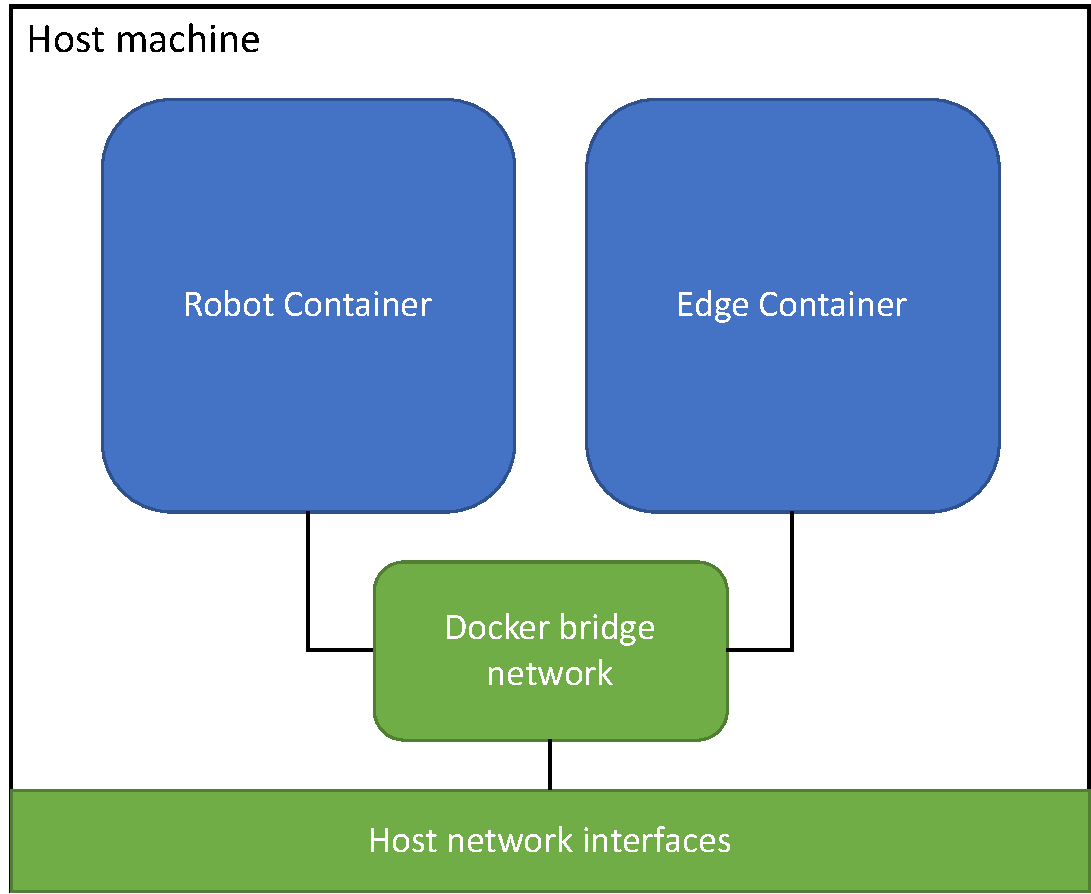
\includegraphics[width=0.6\linewidth]{figures/setup/docker_containers.pdf}
    \caption[Deployment of \gls{docker} containers within the host machine]{This figure shows the deployment of the \gls{docker} containers and the docker bridge network within the host machine. The robot and edge systems are virtualized as \gls{docker} containers. The containers are connected with each other through the \gls{docker} bridge network. The bridge network creates virtual network interfaces for each container.}
    \label{fig:docker_containers}
\end{figure}

The deployment of the docker containers and the docker bridge network within the host machine can be illustrated in \cref{fig:docker_containers}. For \gls{docker} containers, the \gls{cpu} usage can be measured by tools provided by \gls{docker} as well. Since \gls{linux} \gls{docker} containers rely on control groups, \gls{docker} keeps track of the groups of processes of different containers and exposes the metrics, such as \gls{cpu} usage and network IOs. However, container-level CPU energy consumption relies on power estimation models and cannot be directly measured. Moreover, for the specific use case of this thesis, the edge perception is solely calculated using the \gls{gpu}. Therefore, the system-level CPU energy consumption can still reflect the robot's power consumption. Alternatively, the system states of containers can be monitored using \gls{cadvisor}. However, the overhead of such a tool is not negligible. Therefore, it is not adopted as one of the measurement methods. 

For an actual robotic system, the measurements of system states become simple, since the system-level metrics can be directly used. The system states are measured with the "system status" package as a part of the code base of \gls{amsrl}. The "system status" package utilizes the Python package "\gls{psutil}". It can measure system-level CPU usage and CPU power consumption as well as IOs for network interfaces. In the case of Intel \glspl{cpu}, which is used in the work of this thesis exclusively, the power consumption can be measured with \gls{rapl} provided by \gls{linux} kernel Power Capping Framework. The system status node reads the system states and makes them available to the offloading node by publishing them to different \gls{ros} topics. 

Since it is assumed that the edge computer has abundant resources, the system states of the edge computer are not measured and are not taken into consideration during the decision-making and evaluation process. Furthermore, even though only the single-robot single-edge scenario is investigated, the available resources from the edge computers can be affected by numerous factors in real-world applications, such as the number of edge computers, the number of \glspl{amr}, and other processes running the edge computers. In addition, with more powerful hardware and easy access to a power supply, the edge computer consumes more energy and computation resources for the same task than the \gls{amr}'s onboard system. Therefore, it is pointless to compare the consumption of the resources between the two systems. Therefore, only the system states of the \gls{amr}'s onboard system and the network condition between the \gls{amr} and the edge computer are considered.

% For simulation experiments, \gls{docker} provides the containerized system virtualization and virtual network interfaces. \citeauthor*{Ruggeri2022} \cite{Ruggeri2022} proposes that the network bandwidth in use can be measured with the network throughput. The network throughput and \gls{cpu} usage can be measured with the statistics of the \gls{docker} containers, which is a functionality provided by \gls{docker}. Alternatively, the system states of containers can be monitored using \gls{cadvisor}. For real-robot experiments, the \gls{cpu} usage and the network throughput are measured separately on different machines using \gls{psutil} tools. In the case of Intel \glspl{cpu}, the power consumption can be measured with \gls{rapl} provided by \gls{linux} kernel Power Capping Framework. The measurements of CPU usage, network throughput, and power consumption are provided by the "system status" Python package of the code base of \gls{amsrl}. \citeauthor*{Xie2021} \cite{Xie2021} propose that the execution latency of the offloading task consists of two components: the network delay and the inference time. The network delay measures the time needed for transferring the data from the offloading module to the perception module, while the inference time measures the time the perception module needs to process the inference, including the time for image pre-processing and result post-processing. The execution latency is measured with timers residing in the offloading module and the perception module. The timers record the time stamps to critical time points in the transfer and inference process and calculate the time difference. Then, the data are published to a \gls{ros} topic and can be accessed by other subscribers. 

